\documentclass{article}
\usepackage[francais]{babel}
\usepackage[UTF8]{inputenc}
\usepackage[T1]{fontenc}
\usepackage{graphicx}
\usepackage{fancyhdr}
\usepackage{eurosym}
\usepackage{color}
\usepackage{soul}

\pagestyle{fancyplain} \chead{}\lhead{\textit{BLCL}} \rhead{\emph{\textit{ Advanced Tactics}}}

\begin{document}

\thispagestyle{empty}
\begin{center}
 \fontsize{32}{32}{\textbf{ Rapport de soutenance 2 \newline  Advanced Tactics}}
\end{center}

\hspace*{0mm}\vfill
\begin{center}

\includegraphics[scale=0.3]{logo}
\end{center}
\vfill\hspace*{0mm}

\fontsize{14}{14}
\begin{center}
BASTIE \textcolor{red}{"Poutsh"} Arnaud 
\end{center}
\begin{center}
COMMERCON \textcolor{red}{"Uxheal"} Julien
\end{center}
\begin{center}
LAGORCE \textcolor{red}{"Méghane"} Méghane
\end{center}
\begin{center}
LOUVIGNY \textcolor{red}{"TiJack "} Arnaud
\end{center}

\newpage
\thispagestyle{empty}
\tableofcontents

\newpage
\fontsize{12}{12}
\pagenumbering{arabic}
\section{Introduction}

\par
Un peu moins de deux mois se sont écoulés depuis la première soutenance en mars. A cette époque nous n'étions encore que des novices, nous débutions dans le monde du jeu vidéo. Mais depuis, nous avons fait des progrès exceptionnels en matière de programmation et de game design, notre niveau n'a plus rien à voir 
avec celui de nos débuts et tout cela en quelques semaines. Et c'est dans ce rapport que vous allez être témoins de notre avancement dans le projet Advanced Tactics qui, je le rappelle, est un jeu de stratégie tour par tour vu du dessus s'inspirant d'Advance Wars et reprenant les règles des échecs.
\newline

\par
Durant ces deux mois de mars à début mai, nous nous sommes rendus compte que la version de Advanced Tactics de la première soutenance n'était pas à la hauteur, c'est pourquoi nous avons décidé de tout reprendre à zéro afin de créer notre fantastique projet dans les meilleures conditions possibles. Ceci était une initiative
de notre cher partenaire Julien Commerçon et nous le remercions pour cette proposition qui a changé notre manière de créer notre jeu.
\newline

\par
Nous nous sommes très souvent réunis entre les cours pour discuter de Advanced Tactics, partager les tâches et travailler sérieusement sur le projet durant les pauses déjeuner. BLCL Productions n'a jamais été aussi soudé, avant Advanced Tactics nous n'avions pas réellement conscience de ce qu'était le travail d'équipe
mais désormais nous ne travaillons même pas en équipe, nous vivons en équipe. C'est en se serrant les coudes que nous réussirerons à accomplir notre rêve.
\newline

\par
Le projet a donc beaucoup avancé, nous allons justement décrire cet avancement dans ce second rapport de soutenance, le jeu est en bonne voie pour sortir en juin comme prévu. Nous avons fait tester cette version non-commercialisée à des joueurs, nous pouvons vous assurer que cela leur à beaucoup plu. Sur les forums
de jeux vidéo, les joueurs attendent tous Advanced Tactics et pas seulement les férus de jeu de stratégie.
\newline

\par
Nous allons donc enfin vous présenter les nouveautés du jeu, le site internet ainsi que les prévisions pour la prochaine et dernière soutenance.

\newpage



\section{Avancement du projet}

\subsubsection{De nouvelles unités}

\par
Durant notre première soutenance nous n'avions qu'un seul type d'unité, le tank mais qui n'en était pas vraiment un, cela n'était qu'une unité test. Désormais nous possédons une fournée de type d'unité que nous allons vous présenter.
\newline

\par
a)                 Le soldat
\newline

\par
L'unité la plus faible, elle est cependant bon marché et très utile.
\newline

\par
Sprite:
\newline


\includegraphics[scale=1]{soldat}

\par
b)                 Le commando
\newline

\par
Soldat d'élite, bien plus puissant. Il peut vaincre les anti-airs très facilement.
\newline

\par
Sprite:
\newline

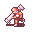
\includegraphics[scale=1]{commando}

\par
c)                 Le tank
\newline

\par
Vous l'avez déjà vu lors de la première soutenance. Il est très puissant et contrairement aux soldats et aux commandos, il peut se déplacer sur les montagnes.
\newline

\par
Sprite:
\newline


\includegraphics[scale=1]{tank}

\par
d)                 L'avion
\newline

\par
L'unité la plus puissante. Elle peut se déplacer sur tous les types de cases en particulier l'eau. Elle est cependant très chère.
\newline

\par
Sprite:
\newline


\includegraphics[scale=1]{avion}

\par
e)                 L'anti-air
\newline

\par
Une sorte de variante du tank. Elle est le point faible des avions.
\newline

\par
Sprite:
\newline


\includegraphics[scale=1]{AA}

\par
f)                 L'ingénieur
\newline

\par
Il peut réparer les véhicules endommagés.
\newline

\par
Sprite:
\newline

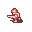
\includegraphics[scale=1]{ing}

\par
g)                 Le médecin
\newline

\par
Il peut soigner les soldats et les commandos.
\newline

\par
Sprite:
\newline


\includegraphics[scale=1]{medic}

\par
h)                 Le camion
\newline

\par
Il peut transporter des unités. Pour ce faire, il faut déplacer l'unité souhaitée sur le camion.
\newline

\par
Sprite:
\newline


\includegraphics[scale=1]{truck}

\newpage

\subsection{Un déplacement et un viseur optmisés}

\par
Le déplacement de la première soutenance était très bancal, peu intuitif et buggé, cependant, il est aujourd'hui grandement amélioré.
\newline

\par
Nous avons fait en sorte que ce soit le plus intuitif possible pour le joueur. Nous utlisions en effet un code couleur bien précis pour le déplacement d'unités, le voici détaillé:
\newline

\par
Lorsque le viseur est blanc, vous n'avez pas encore sélectionné d'unité, vous pouvez le parcourir partout sur la map.
\newline

\par
Par ailleurs nous avons ajouté une petite "feature" concernant le viseur, vous pouvez désormais passer de l'autre côté de la map en appuyant sur une seule touche. Par exemple, imaginons que vous êtes à la dernière ligne de cases en bas, si vous voulez aller à la première ligne de cases en haut,
vous n'avez qu'à appuyer sur la flèche du bas tout simplement. Pareil pour la droite et la gauche. Cela permet de rendre la navigation beaucoup plus fluide et par conséquent d'améliorer le confort du joueur, chose indispensable dans un jeu de stratégie.
\newline

\par
Sprite du viseur blanc:
\newline


\includegraphics[scale=1]{blanc}

\newline

\par
Lorsque vous sélectionnez l'unité en appuyant sur la touche Q, un viseur jaune apparait autour de l'unité sélectionnée. Cela permet au joueur de bien se rappeler quelle unité il a choisi de déplacer.
\newline

\par
Sprite du viseur jaune:
\newline


\includegraphics[scale=1]{jaune}

\newline

\par
Vous pouvez maintenant déplacer l'unité en sélectionnant sa nouvelle position avec la touche Q. Cependant, l'unité ne peut bien entendu pas se déplacer partout, tout cela varie en fonction de sa classe (pion, fou dame...) et en fonction du type de terrain.
\newline

\par
Lorsque vous pouvez déplacer l'unité sur une case, le viseur est bleu.
\newline

\par
Sprite du viseur bleu:
\newline


\includegraphics[scale=1]{bleu}

\newline

\par
Lorsque vous ne pouvez déplacer l'unité sur une case, le viseur est rouge.
\newline

\par
Sprite du viseur rouge:
\newline


\includegraphics[scale=1]{rouge}

\newpage

\subsection{Un nouveau scénario}

\par
Le scénario de Advanced Tactics avait jusque là été assez pauvre, nous nous concentrions esstiellement sur le gameplay car comme le dit souvent le grand Shigeru Miyamoto, il faut toujours d'abord penser au gameplay dans un jeu vidéo. Cependant, nous sommes conscients de l'importance du scénario ainsi
que du background dans un jeu vidéo, c'est quelque chose qui intéresse fortement les joueurs, surtout de nos jours, et donc un point absolument pas négligeable, surtout dans un jeu de stratégie basé sur la guerre. Nous avons repris les bases de l'ancien petit scénario de Advanced Tactics mais l'avons grandement
amélioré, c'est dans cette partie que nous allons vous le présenter.
\newline

\par
Le pétrole est complètement épuisé sur Terre depuis 2045. Pendant des dizaines d'années les hommes pauvres ont souffert à cause de ce manque d'énergie. Mais une nouvelle forme d'énergie a été découverte sur la planète Mars, on l'appelle le Kalder. C'est un pouvoir incroyable laissé par une ancienne
civilisation martienne et qui permet toutes sortes de choses extraordinaires telles que la téléportation. Cependant cette énergie reste tout de même extrêmement rare.
\newline

\par
2189. Le Kalder a apporté énormément de bien pour l'humanité mais certaines personnes avec de mauvaises intentions l'ont utliisé pour faire le mal. C'est le cas du général Reinhard von Köruschbool qui s'est servi du Kalder pour faire un coup d'état dans le puissant empire Bläckorsch. Il dirige une grande partie
du monde et mène une dictature totalitaire d'un niveau encore jamais atteint même dans les heures les plus sombres de notre histoire. Cet homme est le mal incarné, il a une obsession envers la force et l'intelligence des gens, c'est pourquoi, il procède à plusieurs sortes de génocide des personnes faibles dans 
son empire. Rien ne semble arreter l'expansion de son domaine, la plupart des gens pensent qu'il arrivera à dominer le monde. Car Reinhard von Köruschbool est un génie de la guerre, l'un des plus grands de toute l'histoire.
\newline

\par
La petite république européenne de Whärschtoph va bientot se faire envahir par l'empire Bläckorsch. Son peuple est désespéré, les dirigeants pensent à se rendre avant même qu'une bataille commence. Mais, il existe un espoir. En effet, un jeune étudiant des écoles de stratégies militaires est tout simplement
surdoué. Ses professeurs affirment qu'il dépasse de très loin le niveau déjà exceptionnel du général Reinhard von Köruschbool. Les dirigeants de la république Whärschtoph compent alors lui donner les rennes de la stratégie militaire du pays. Cet étudiant, c'est vous.
\newline

\par
Mais les batailles militaires ne se déroulent plus comme avant en 2189. En effet, pour limiter les morts, il n'y a plus d'humains sur le champ de bataille, les soldats ont été remplacés en 2124 par des cyborgs ultra perfectionnés qui marchent grâce à l'énergie Kalder. Il y a également des véhicules automatiques très
puissant. Les unités qui marchent au Kalder ne se déplacent donc plus en avançant, la téléportation est devenue l'outil principal du déplacement militaire grâce au Kalder. Mais cette énergie étant très chère, les téléportations ne sont pas infinies, sa portée est donc limitée selon les unités. Sur le champ de bataille
il y a en réalité deux humains, les deux généraux qui s'affrontent et qui dirigent toutes leurs unités sur un grand tableau de bord comme dans un jeu de plateau. On appelle cela la technologie Advanced Tactics. C'est de là d'où vient le titre du projet et en réalité le jeu lui-même représente le tableau de bord du
stratège que vous incarnez.
\newline

\par
Le héros de Advanced Tactics est très amitieux. Il ne compte pas simplement protéger sa patrie mais il souhaite faire tomber le régime totalitaire horrible du général Reinhard von Körsuchbool en attaquant directement la capitale de l'empire Bläckorsch où se trouve le siège du pouvoir: Hepïtarh. La fantastique aventure
Advanced Tactics commence.
\newline

\newpage

\begin{center}
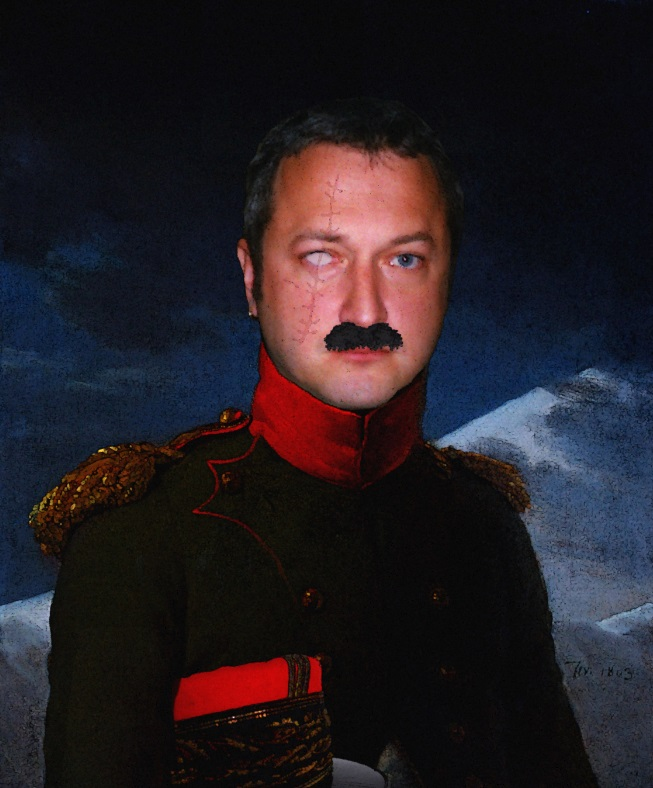
\includegraphics[scale = 1]{général}
\newline
\par
Le portrait du général Reinhard Von Köruschbool.
\end{center}

\newpage

\subsection{La Map}

\par
Les nouvelles maps de Advanced Tactics n'ont plus rien à voir avec la pauvre map minuscule de la première soutenance, nous avons beaucoup avancé sur ce domaine du jeu.
\newline

\par
Tout d'abord, les maps peuvent avoir un nombre infini de tailles. Auparavant, les maps ne pouvaient que que faire 20 cases sur 20 cases, cela était très dérangeant, et les possibilités de jeu étaient limités. Jouer sur un grand champ de bataille est bien plus immersif et épique.
\newline

\par
Mais la plus grande avancée sur les maps c'est sans aucun doute notre éditeur de map tout simplement exceptionnel.
\newline

\par
Pour des maps aussi grandes que celles de Advanced Tactics, remplir case par case avec des terrains différents dans l'éditeur serait laborieux, pas du tout amusant pour le joueur et il aurait plus de chance de faire une map incohérente et mal designé. Cela marchait bien avec notre ancien éditeur de map
quand la taille de nos maps était limitée à 20 cases par 20 cases mais cela ne pouvait plus continuer comme ça, nous avons donc créé un tout nouvel éditeur de map extrêmement performant qui n'a plus rien à voir avec l'ancien.
\newline

\par
Cet éditeur de map est assez spécial. Sa particulirarité, c'est qu'il permet de créer de manière très simple et très rapide de la cohérence dans la géographie.
\newline

\par
Voici son fonctionnement. Avec les boutons de la série, placez des reliefs montagnez ou des plaines, qui s'affichent toujours de manière cohérente et réaliste.
\newline

\par
Puis après, gérez le niveau de la mer grâce à la molette de la souris. Vous obtiendrez toujours une map très belle avec un bon level design que vous pouvez réaliser en quelques secondes.
\newline

\par
Lorsque vous quittez l'éditeur, la map que vous avez créé se sauvegarde et lorsque vous lancez Advanced Tactics, vous jouez directement avec cette map.
\newline

\newpage

\begin{center}
\includegraphics[scale=0.5]{mapedit1}
\newline
\par
La map sur l'éditeur.
\newline
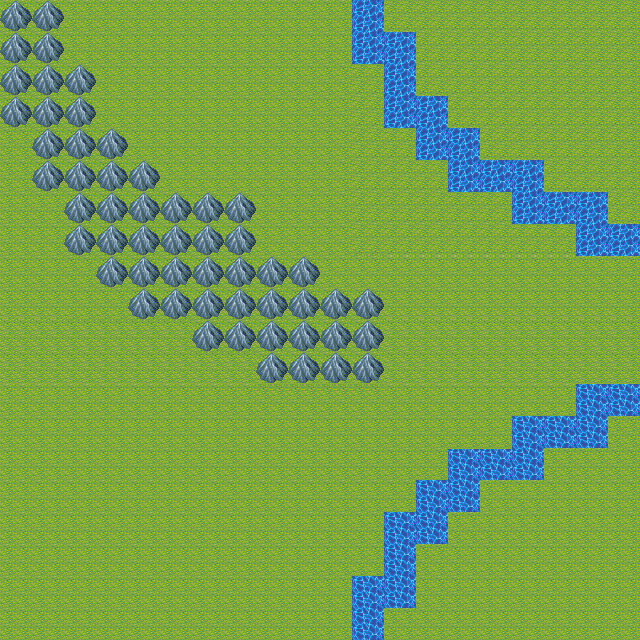
\includegraphics[scale=0.5]{map1}
\newline
\par
La map en jeu.
\end{center}

\newpage

\begin{center}
\includegraphics[scale=0.5]{mapedit2}
\newline
\par
La map sur l'éditeur.
\newline
\includegraphics[scale=0.5]{map2}
\newline
\par
La map en jeu.
\end{center}

\newpage

\subsection{Un tableau de bord dynamique}

\par
Le "tableau de bord dynamique" est un outil très important dans un jeu de stratégie car il permet au joueur d'avoir très rapidement beaucoup d'informations qui s'affichent en temps réel dans son menu, celui de Advanced Tactilcs est très utile.
\newline

\par
En effet à gauche de l'écran, sur un très beau fond métallisé, vous pouvez voir plusieurs informations qui s'affichent dynamiquement en fonction de la position du viseur.
\newline

\par
Vous pouvez donc respectivement voir:
\newline

\par
Les coordonnées de la case où se situe le viseur.
\newline

\par
Le type de terrain de la case où se situe le viseur, terre, mer ou montagne.
\newline

\par
Si une unité est présente vous pouvez voir son type, son sprite, ses points de vie, et sa force.
\newline

\newpage

\par
Voici plusieurs images du tableau de bord dynamique:
\newline

\begin{center}
\includegraphics[scale=1]{menu1}
\newline
\includegraphics[scale=1]{menu2}
\newline
\includegraphics[scale=1]{menu3}
\newline
\end{center}

\newpage

\subsection{Des combats d'unités}

\par
C'était une avancée indispensable de Advanced Tactics. Vous pouvez désormais enfin attaquer des unités.
\newline

\par
Pour ce faire, cela fonctionne un peu comme le déplacement, vous sélectionnez l'unité de votre choix puis vous choisissez l'unité à attaquer. Il faut qu'elle soit dans la portée de l'unité sélectionnée.
\newline

\par
Lorsque vous attaquez, l'unité perd des PV, lorsque ceux-ci arrivent à zéro, l'unité est détruite dans une grosse explosion
\newline

\begin{center}
\includegraphics[scale=1]{attaque}
\par
Une unité meurt.
\newline
\end{center}

\newpage

\subsection{Des animations et des sons}

\par
L'immersion est un point très important dans le jeu vidéo. Il faut que le joueur s'imprègne dans l'ambiance du jeu et se sente impliqué grâce à cela.
\newline

\par
C'est pourquoi nous avons ajouté des animations et des sons quand une unité se téléporte ou explose.
\newline

\begin{center}
\includegraphics[scale=1]{téléport}
\par
Une unité se téléporte.
\newline
\end{center}

\newpage

\begin{center}
\includegraphics[scale=0.6]{prog}
\par
Advanced Tactics en pleine programmation.
\newline
\end{center}

\section{Et après...}

\par
Nous avons très bien avancé sur le projet pour cette soutenance mais le jeu va bientot sortir et nous allons devoir entièrement le finir.
\newline

\subsection{Les futurs nouveaux ajouts}

\par
Voici ce que nous comptons ajouter par la suite:
\newline

\par
-Une unité camion fonctionnelle
\newline

\par
-La gestion du tour par tour avec les deux camps
\newline

\par
-Le multijoueur sur un écran et en réseau
\newline

\par
-L'intelligence artificielle
\newline

\par
-Finition du magasin
\newline

\newpage

\section{Le site Internet}

\par
Nous avons désormais un site Internet!
\newline

\par
Voici l'adresse du site:
\newline

\par
Le voici en images:
\newline

\begin{center}
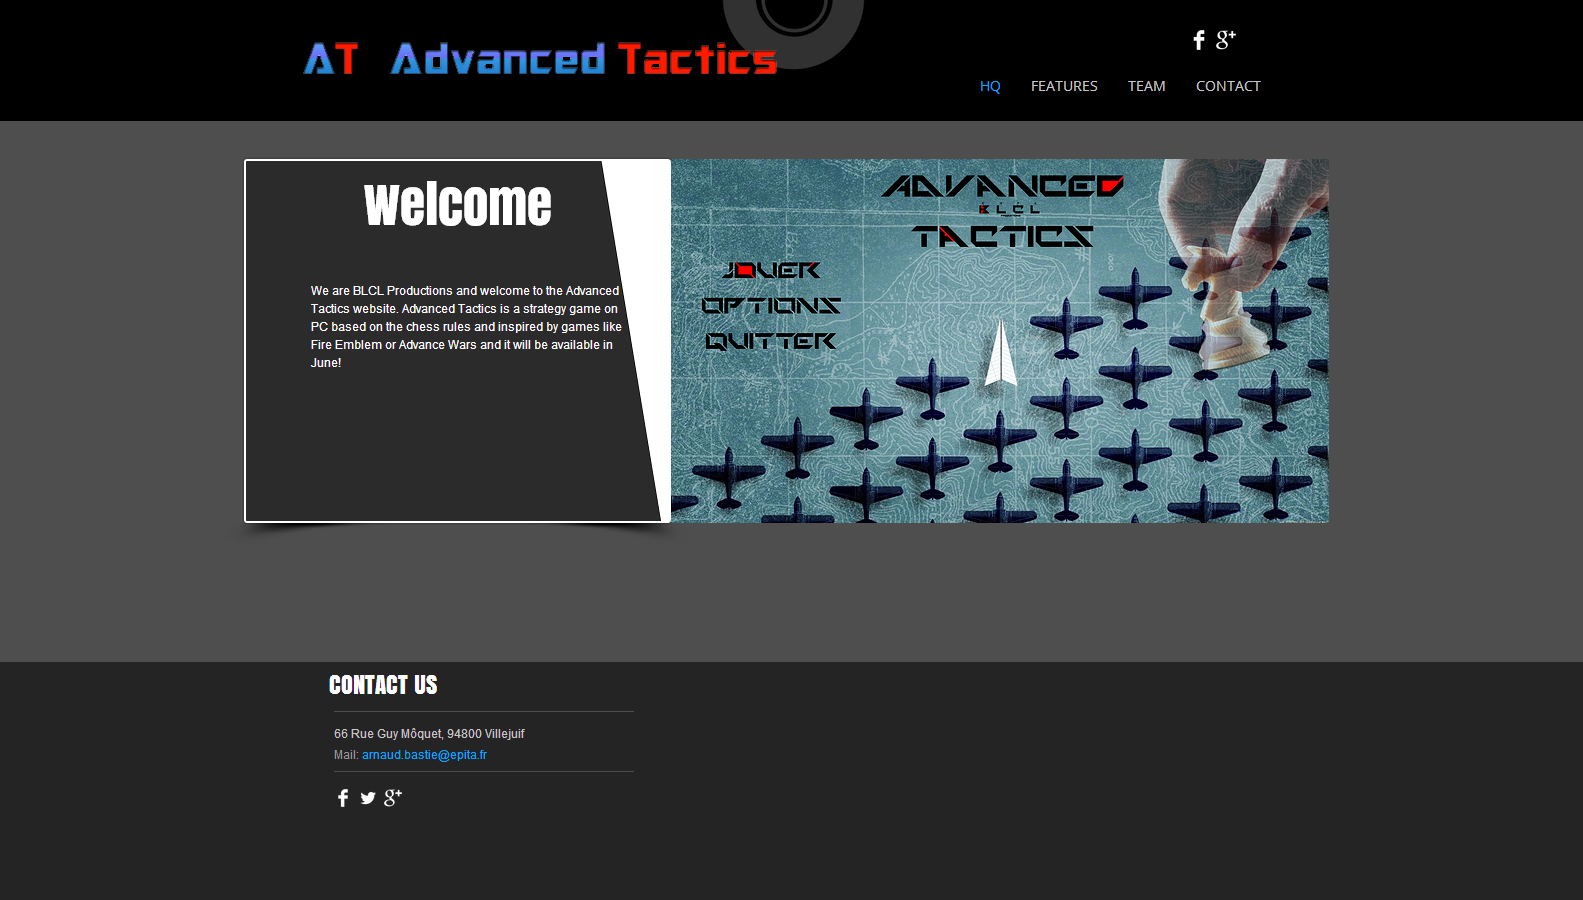
\includegraphics[scale=1]{site}
\par
La page d'accueil du site Internet de Advanced Tactics
\newline
\end{center}

\newpage

\section{Conclusion}
\par
Ces mois nous ont prouvé que nous avons fait énormément de progrès. Advanced Tactics est en bonne voie pour devenir un excellent jeu de stratégie.

\end{document}
